\hypertarget{the-auditory-and-vestibular-systems}{%
\chapter{The Auditory And Vestibular Systems}\label{the-auditory-and-vestibular-systems}}

The auditory system is the sensory system for the sense of hearing. It includes both the sensory organs (the ears) and the auditory parts of the sensory system. Hearing, or auditory perception, is the ability to perceive sounds by detecting vibrations, changes in the pressure of the surrounding medium over time, through the ear.

Providing balance, when moving or stationary, is also a central function of the ear. The ear facilitates two types of balance: static balance, which allows a person to feel the effects of gravity, and dynamic balance, which allows a person to sense acceleration.

\hypertarget{the-ear}{%
\section{The Ear}\label{the-ear}}

In mammals, the ear is usually described as having three parts---the outer ear, the middle ear and the inner ear. The outer ear consists of the pinna and the ear canal. The folds of cartilage surrounding the ear canal are called the pinna. Sound waves are reflected and attenuated when they hit the pinna, and these changes provide additional information that will help the brain determine the sound direction. Since the outer ear is the only visible portion of the ear in most animals, the word ``ear'' often refers to the external part alone. The middle ear includes the tympanic cavity and the three ossicles. The inner ear sits in the bony labyrinth, and contains structures which are key to several senses: the semicircular canals, which enable balance and eye tracking when moving; the utricle and saccule, which enable balance when stationary; and the cochlea, which enables hearing. The ears of vertebrates are placed somewhat symmetrically on either side of the head, an arrangement that aids sound localisation.

The ear develops from the first pharyngeal pouch and six small swellings that develop in the early embryo called otic placodes, which are derived from ectoderm.

The ear canal of the outer ear is separated from the air-filled tympanic cavity of the middle ear by the eardrum. The middle ear contains the three small bones---the ossicles---involved in the transmission of sound, and is connected to the throat at the nasopharynx, via the pharyngeal opening of the Eustachian tube. The inner ear contains the otolith organs---the utricle and saccule---and the semicircular canals belonging to the vestibular system, as well as the cochlea of the auditory system.



\begin{figure}

{\centering 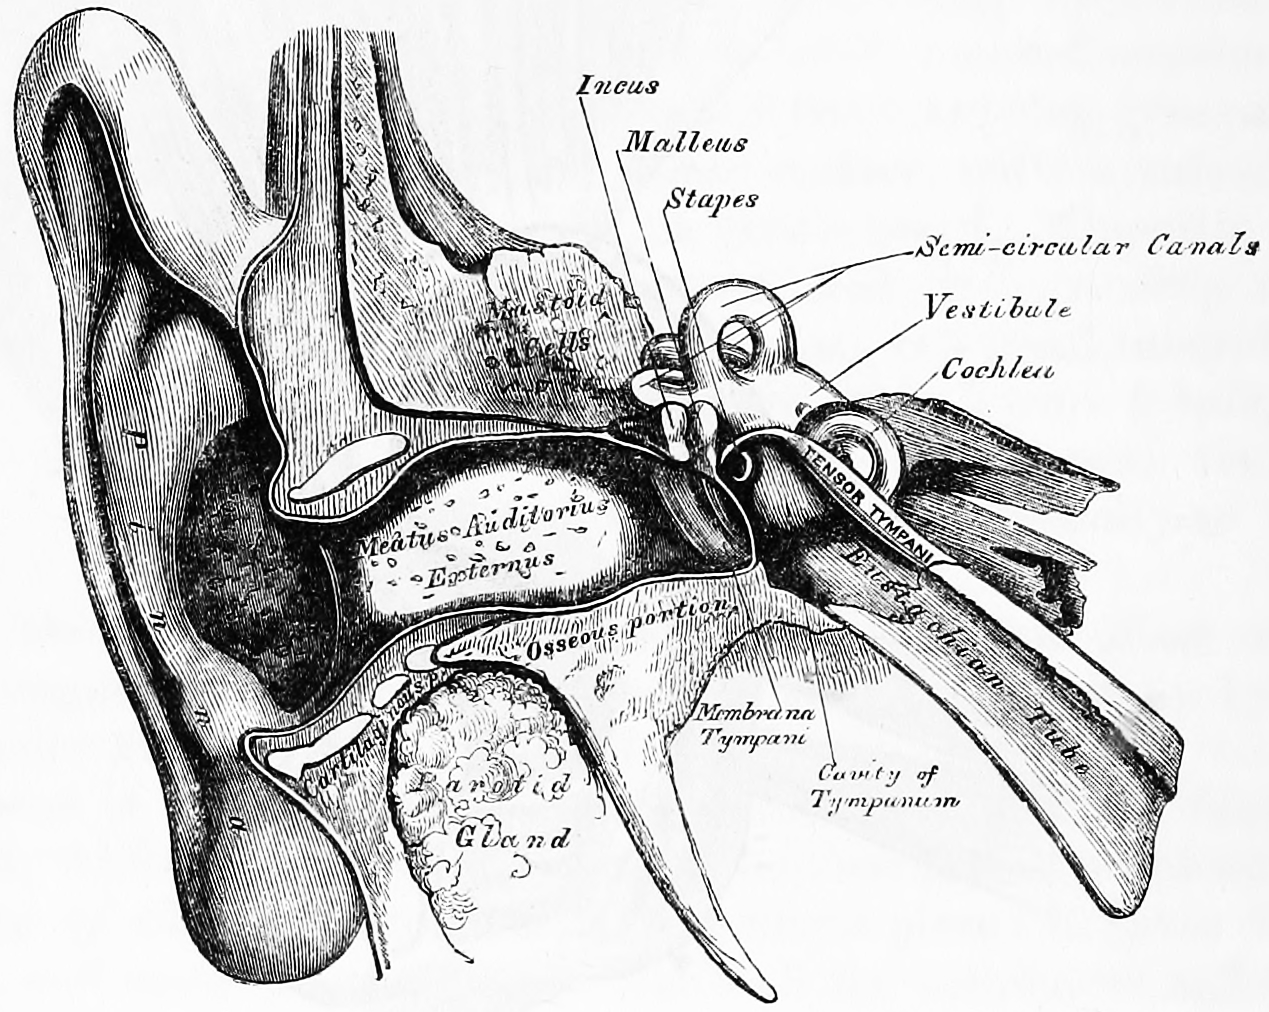
\includegraphics[width=0.7\linewidth]{./figures/auditory/GrayEar} 

}

\caption{Front view of the right outer, middle and inner ear. \href{https://archive.org/details/anatomydescripti00grayuoft/page/n6/mode/2up}{Gray, Henry, 1825-1861. Anatomy, descriptive and surgical; ed.~by T. Pickering Pick and Robert Howden. A revised American, from the fifteenth English edition. Philadelphia, Lea, 1901}}\label{fig:rightear}
\end{figure}

Sound waves travel through the ear canal and hit the tympanic membrane, or eardrum. This wave information travels across the air-filled middle ear cavity via a series of delicate bones: the malleus (hammer), incus (anvil) and stapes (stirrup). These ossicles act as a lever, converting the lower-pressure eardrum sound vibrations into higher-pressure sound vibrations at another, smaller membrane called the oval window or vestibular window. The manubrium (handle) of the malleus articulates with the tympanic membrane, while the footplate (base) of the stapes articulates with the oval window. Higher pressure is necessary at the oval window than at the typanic membrane because the inner ear beyond the oval window contains liquid rather than air. The stapedius reflex of the middle ear muscles helps protect the inner ear from damage by reducing the transmission of sound energy when the stapedius muscle is activated in response to sound. The middle ear still contains the sound information in wave form; it is converted to nerve impulses in the cochlea.
The middle-ear ossicles further amplify the vibration pressure roughly 20 times. The base of the stapes couples vibrations into the cochlea via the oval window, which vibrates the perilymph liquid (present throughout the inner ear) and causes the round window to bulb out as the oval window bulges in.

The inner ear consists of the cochlea and several non-auditory structures. The cochlea has three fluid-filled sections (i.e.~the scala media, scala tympani and scala vestibuli), and supports a fluid wave driven by pressure across the basilar membrane separating two of the sections. Strikingly, one section, called the cochlear duct or scala media, contains endolymph. Endolymph is a fluid similar in composition to the intracellular fluid found inside cells. The organ of Corti is located in this duct on the basilar membrane, and transforms mechanical waves to electric signals in neurons. The other two sections are known as the scala tympani and the scala vestibuli. These are located within the bony labyrinth, which is filled with fluid called perilymph, similar in composition to cerebrospinal fluid. The chemical difference between the fluids endolymph and perilymph fluids is important for the function of the inner ear.

\hypertarget{the-auditory-system}{%
\section{The Auditory System}\label{the-auditory-system}}

In humans and other vertebrates, hearing is performed primarily by the auditory system: mechanical waves, known as vibrations, are detected by the ear and transduced into nerve impulses that are perceived by the brain (primarily in the temporal lobe). Like touch, audition requires sensitivity to the movement of molecules in the world outside the organism. Both hearing and touch are types of mechanosensation. Sound may be heard through solid, liquid, or gaseous matter. It is one of the traditional five senses; partial or total inability to hear is called hearing loss.

\hypertarget{organ-of-corti}{%
\subsection{Organ Of Corti}\label{organ-of-corti}}

The organ of Corti, or spiral organ, is the receptor organ for hearing and is located in the mammalian cochlea. This highly varied strip of epithelial cells allows for transduction of auditory signals into nerve impulses. Transduction occurs through vibrations of structures in the inner ear causing displacement of cochlear fluid and movement of hair cells at the organ of Corti to produce electrochemical signals.

Italian anatomist \href{https://en.wikipedia.org/wiki/Alfonso_Giacomo_Gaspare_Corti}{Alfonso Giacomo Gaspare Corti} (1822--1876) discovered the organ of corti in 1851.

The organ of corti is located in the scala media of the cochlea of the inner ear between the vestibular duct and the tympanic duct and is composed of mechanosensory cells, known as hair cells. strategically positioned on the basilar membrane of the organ of corti are three rows of outer hair cells (ohcs) and one row of inner hair cells (ihcs). Separating these hair cells are supporting cells: Deiters cells, also called phalangeal cells, which separate and support both the ohcs and the ihcs.



\begin{figure}

{\centering 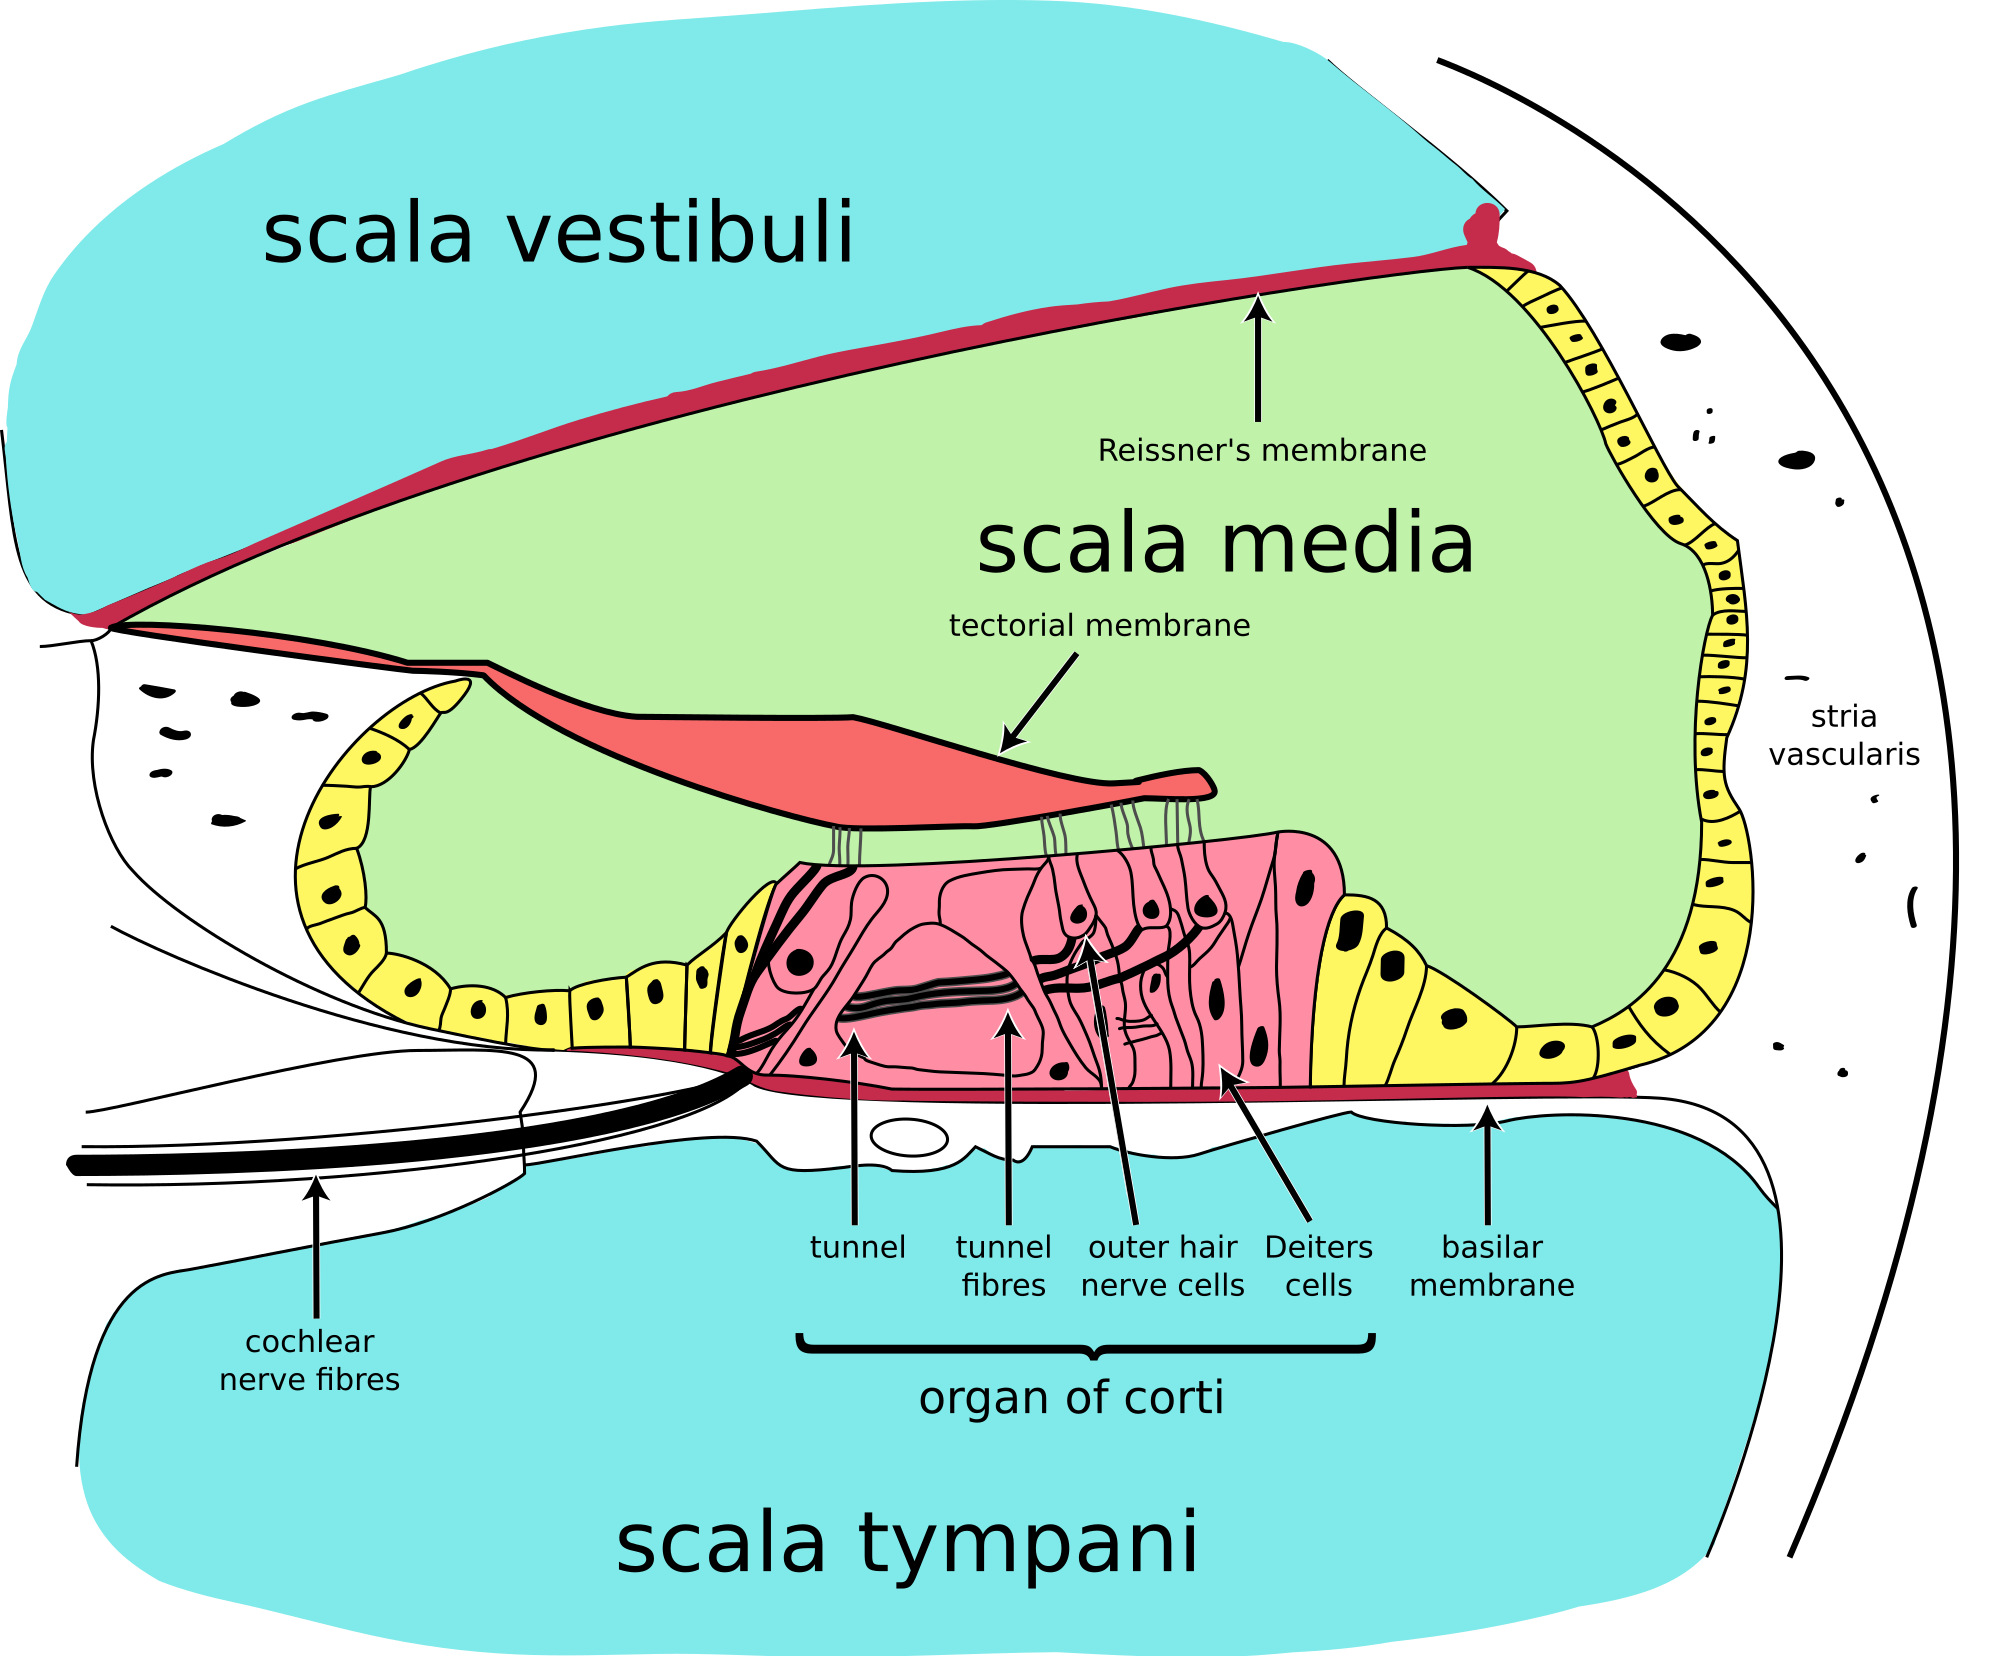
\includegraphics[width=0.7\linewidth]{./figures/auditory/Cochlea-crosssection} 

}

\caption{\href{https://commons.wikimedia.org/wiki/File:Cochlea-crosssection.svg}{A cross section of the cochlea illustrating the organ of Corti.}}\label{fig:organcorti}
\end{figure}

Projecting from the tips of the hair cells are tiny finger like projections called stereocilia, which are arranged in a graduated fashion with the shortest stereocilia on the outer rows and the longest in the center.

If the cochlea were uncoiled it would roll out to be about 33 mm long in women and 34 mm in men, with about 2.28 mm of standard deviation for the population. The cochlea is also tonotopically organized, meaning that different frequencies of sound waves interact with different locations on the structure. The base of the cochlea, closest to the outer ear, is the most stiff and narrow and is where the high frequency sounds are transduced. The apex, or top, of the cochlea is wider and much more flexible and loose and functions as the transduction site for low frequency sounds.

\hypertarget{auditory-transduction}{%
\subsection{Auditory Transduction}\label{auditory-transduction}}

In normal hearing subjects, the majority of the auditory signals that reach the organ of Corti in the first place come from the outer ear. Sound waves enter through the auditory canal and vibrate the tympanic membrane, also known as the eardrum, which vibrates three small bones called the ossicles. As a result, the attached oval window moves and causes movement of the round window, which leads to displacement of the cochlear fluid. However, the stimulation can happen also via direct vibration of the cochlea from the skull. The latter is referred to as Bone Conduction (or BC) hearing, as complementary to the first one described, which is instead called Air Conduction (or AC) hearing. Both AC and BC stimulate the basilar membrane in the same way.

The basilar membrane on the tympanic duct presses against the hair cells of the organ as perilymphatic pressure waves pass. The stereocilia atop the IHCs move with this fluid displacement and in response their cation, or positive ion selective, channels are pulled open by cadherin structures called tip links that connect adjacent stereocilia. The organ of Corti, surrounded in potassium rich fluid endolymph, lies on the basilar membrane at the base of the scala media. Under the organ of Corti is the scala tympani and above it, the scala vestibuli. Both structures exist in a low potassium fluid called perilymph. Because those stereocilia are in the midst of a high concentration of potassium, once their cation channels are pulled open, potassium ions as well as calcium ions flow into the top of the hair cell. With this influx of positive ions the IHC becomes depolarized, opening voltage-gated calcium channels at the basolateral region of the hair cells and triggering the release of the neurotransmitter glutamate. An electrical signal is then sent through the auditory nerve and into the auditory cortex of the brain as a neural message.

The organ of Corti is also capable of modulating the auditory signal. The outer hair cells (OHCs) can amplify the signal through a process called electromotility where they increase movement of the basilar and tectorial membranes and therefore increase deflection of stereocilia in the IHCs.

A crucial piece to this cochlear amplification is the motor protein prestin, which changes shape based on the voltage potential inside of the hair cell. When the cell is depolarized, prestin shortens, and because it is located on the membrane of OHCs it then pulls on the basilar membrane and increasing how much the membrane is deflected, creating a more intense effect on the inner hair cells (IHCs). When the cell hyperpolarizes prestin lengthens and eases tension on the IHCs, which decreases the neural impulses to the brain. In this way, the hair cell itself is able to modify the auditory signal before it even reaches the brain.

Hair cells are columnar cells, each with a bundle of 100--200 specialized cilia at the top, for which they are named. There are two types of hair cells; inner and outer hair cells. Inner hair cells are the mechanoreceptors for hearing: they transduce the vibration of sound into electrical activity in nerve fibers, which is transmitted to the brain. Outer hair cells are a motor structure. Sound energy causes changes in the shape of these cells, which serves to amplify sound vibrations in a frequency specific manner. Lightly resting atop the longest cilia of the inner hair cells is the tectorial membrane, which moves back and forth with each cycle of sound, tilting the cilia, which is what elicits the hair cells' electrical responses.

Inner hair cells, like the photoreceptor cells of the eye, show a graded response, instead of the spikes typical of other neurons.

\hypertarget{auditory-pathways}{%
\subsection{Auditory Pathways}\label{auditory-pathways}}

Afferent neurons innervate cochlear inner hair cells, at synapses where the neurotransmitter glutamate communicates signals from the hair cells to the dendrites of the primary auditory neurons.

There are far fewer inner hair cells in the cochlea than afferent nerve fibers -- many auditory nerve fibers innervate each hair cell. The neural dendrites belong to neurons of the auditory nerve, which in turn joins the vestibular nerve to form the vestibulocochlear nerve, or cranial nerve number VIII. The region of the basilar membrane supplying the inputs to a particular afferent nerve fibre can be considered to be its receptive field.

Efferent projections from the brain to the cochlea also play a role in the perception of sound, although this is not well understood. Efferent synapses occur on outer hair cells and on afferent (towards the brain) dendrites under inner hair cells

\hypertarget{the-cochlear-nucleus}{%
\subsection{The Cochlear Nucleus}\label{the-cochlear-nucleus}}

The cochlear nucleus is the first site of the neuronal processing of the newly converted ``digital'' data from the inner ear. In mammals, this region is anatomically and physiologically split into two regions, the dorsal cochlear nucleus (DCN), and ventral cochlear nucleus (VCN). The VCN is further divided by the nerve root into the posteroventral cochlear nucleus (PVCN) and the anteroventral cochlear nucleus (AVCN).

\hypertarget{the-trapezoid-body}{%
\subsection{The Trapezoid Body}\label{the-trapezoid-body}}

The trapezoid body is a bundle of decussating fibers in the ventral pons that carry information used for binaural computations in the brainstem. Some of these axons come from the cochlear nucleus and cross over to the other side before traveling on to the superior olivary nucleus. This is believed to help with localization of sound.

\hypertarget{the-superior-olivary-complex}{%
\subsection{The superior olivary complex}\label{the-superior-olivary-complex}}

The superior olivary complex is located in the pons, and receives projections predominantly from the ventral cochlear nucleus, although the dorsal cochlear nucleus projects there as well, via the ventral acoustic stria. Within the superior olivary complex lies the lateral superior olive (LSO) and the medial superior olive (MSO). The former is important in detecting interaural level differences while the latter is important in distinguishing interaural time difference.

\hypertarget{the-lateral-lemniscus}{%
\subsection{The Lateral Lemniscus}\label{the-lateral-lemniscus}}

The lateral lemniscus is a tract of axons in the brainstem that carries information about sound from the cochlear nucleus to various brainstem nuclei and ultimately the contralateral inferior colliculus of the midbrain.

\hypertarget{the-inferior-colliculi}{%
\subsection{The Inferior Colliculi}\label{the-inferior-colliculi}}

The inferior colliculi (IC) are located just below the visual processing centers known as the superior colliculi. The central nucleus of the IC is a nearly obligatory relay in the ascending auditory system, and most likely acts to integrate information (specifically regarding sound source localization from the superior olivary complex and dorsal cochlear nucleus) before sending it to the thalamus and cortex.

\hypertarget{the-medial-geniculate-nucleus-mgn}{%
\subsection{The Medial Geniculate Nucleus (MGN)}\label{the-medial-geniculate-nucleus-mgn}}

The medial geniculate nucleus is part of the thalamic relay system.

\hypertarget{the-primary-auditory-cortex}{%
\subsection{The Primary Auditory Cortex}\label{the-primary-auditory-cortex}}

The primary auditory cortex is the first region of cerebral cortex to receive auditory input.

Perception of sound is associated with the left posterior superior temporal gyrus (STG). The superior temporal gyrus contains several important structures of the brain, including Brodmann areas 41 and 42, marking the location of the primary auditory cortex, the cortical region responsible for the sensation of basic characteristics of sound such as pitch and rhythm. We know from research in nonhuman primates that the primary auditory cortex can probably be divided further into functionally differentiable subregions. The neurons of the primary auditory cortex can be considered to have receptive fields covering a range of auditory frequencies and have selective responses to harmonic pitches. Neurons integrating information from the two ears have receptive fields covering a particular region of auditory space.

The primary auditory cortex is surrounded by secondary auditory cortex, and interconnects with it. These secondary areas interconnect with further processing areas in the superior temporal gyrus, in the dorsal bank of the superior temporal sulcus, and in the frontal lobe. In humans, connections of these regions with the middle temporal gyrus are probably important for speech perception. The frontotemporal system underlying auditory perception allows us to distinguish sounds as speech, music, or noise.

\hypertarget{the-auditory-ventral-and-dorsal-streams}{%
\subsection{The Auditory Ventral And Dorsal Streams}\label{the-auditory-ventral-and-dorsal-streams}}

From the primary auditory cortex emerge two separate pathways: the auditory ventral stream and auditory dorsal stream. The auditory ventral stream includes the anterior superior temporal gyrus, anterior superior temporal sulcus, middle temporal gyrus and temporal pole. Neurons in these areas are responsible for sound recognition, and extraction of meaning from sentences. The auditory dorsal stream includes the posterior superior temporal gyrus and sulcus, inferior parietal lobule and intra-parietal sulcus. Both pathways project in humans to the inferior frontal gyrus. The most established role of the auditory dorsal stream in primates is sound localization. In humans, the auditory dorsal stream in the left hemisphere is also responsible for speech repetition and articulation, phonological long-term encoding of word names, and verbal working memory.

\hypertarget{the-vestibular-system}{%
\section{The Vestibular System}\label{the-vestibular-system}}

The vestibular system, in vertebrates, is part of the inner ear. In most mammals, the vestibular system is the sensory system that provides the leading contribution to the sense of balance and spatial orientation for the purpose of coordinating movement with balance. Together with the cochlea, a part of the auditory system, it constitutes the labyrinth of the inner ear in most mammals. As movements consist of rotations and translations, the vestibular system comprises two components: the semicircular canals which indicate rotational movements; and the otoliths which indicate linear accelerations. The vestibular system sends signals primarily to the neural structures that control eye movements, and to the muscles that keep an animal upright and in general control posture. The projections to the former provide the anatomical basis of the vestibulo-ocular reflex, which is required for vision; while the projections to the latter provide the anatomical means required to enable an animal to maintain its position in space.

The brain uses information from the vestibular system in the head and from proprioception throughout the body to enable the animal to understand its body's dynamics and kinematics (including its position and acceleration) from moment to moment. How these two perceptive sources are integrated to provide the underlying structure of the sensorium is unknown.

\hypertarget{the-semicircular-canals}{%
\subsection{The Semicircular Canals}\label{the-semicircular-canals}}

The semicircular canal system detects rotational movements.

The semicircular canals are a component of the bony labyrinth that are at right angles to each other. At one end of each of the semicircular canals is a dilated sac called an osseous ampulla which is more than twice the diameter of the canal. Each ampulla contains an ampulla crest, the crista ampullaris which consists of a thick gelatinous cap called a cupula and many hair cells. The superior and posterior semicircular canals are oriented vertically at right angles to each other. The lateral semicircular canal is about a 30-degree angle from the horizontal plane. The orientations of the canals cause a different canal to be stimulated by movement of the head in different planes, and more than one canal is stimulated at once if the movement is off those planes. The horizontal canal detects angular acceleration of the head when the head is turned and the superior and posterior canals detect vertical head movements when the head is moved up or down. When the head changes position, the endolymph in the canals lags behind due to inertia and this acts on the cupula which bends the cilia of the hair cells. The stimulation of the hair cells sends the message to the brain that acceleration is taking place. The ampullae open into the vestibule by five orifices, one of the apertures being common to two of the canals.

Since the world is three-dimensional, the vestibular system contains three semicircular canals in each labyrinth. They are approximately orthogonal (at right angles) to each other, and are the horizontal (or lateral), the anterior semicircular canal (or superior), and the posterior (or inferior) semicircular canal. Anterior and posterior canals may collectively be called vertical semicircular canals.

The anterior and posterior semicircular canals detect rotations of the head in the sagittal plane (as when nodding), and in the frontal plane, as when cartwheeling. Both anterior and posterior canals are orientated at approximately 45° between frontal and sagittal planes.
The movement of fluid pushes on a structure called the cupula which contains hair cells that transduce the mechanical movement to electrical signals.

The canals are arranged in such a way that each canal on the left side has an almost parallel counterpart on the right side. Each of these three pairs works in a push-pull fashion: when one canal is stimulated, its corresponding partner on the other side is inhibited, and vice versa.

\hypertarget{the-otolithic-organs}{%
\subsection{The Otolithic Organs}\label{the-otolithic-organs}}

While the semicircular canals respond to rotations, the otolithic organs sense linear accelerations. Humans have two otolithic organs on each side, one called the utricle, the other called the saccule. The utricle contains a patch of hair cells and supporting cells called a macula. Similarly, the saccule contains a patch of hair cells and a macula. Each hair cell of a macula has 40-70 stereocilia and one true cilium called a kinocilium. The tips of these cilia are embedded in an otolithic membrane. This membrane is weighted down with protein-calcium carbonate granules called otoconia. These otoconia add to the weight and inertia of the membrane and enhance the sense of gravity and motion. With the head erect, the otolithic membrane bears directly down on the hair cells and stimulation is minimal. When the head is tilted, however, the otolithic membrane sags and bends the stereocilia, stimulating the hair cells. Any orientation of the head causes a combination of stimulation to the utricles and saccules of the two ears. The brain interprets head orientation by comparing these inputs to each other and to other input from the eyes and stretch receptors in the neck, thereby detecting whether the head is tilted or the entire body is tipping. Essentially, these otolithic organs sense how quickly you are accelerating forward or backward, left or right, or up or down. Most of the utricular signals elicit eye movements, while the majority of the saccular signals projects to muscles that control our posture.

While the interpretation of the rotation signals from the semicircular canals is straightforward, the interpretation of otolith signals is more difficult: since gravity is equivalent to a constant linear acceleration, one somehow has to distinguish otolith signals that are caused by linear movements from those caused by gravity. Humans can do that quite well, but the neural mechanisms underlying this separation are not yet fully understood. Humans can sense head tilting and linear acceleration even in dark environments because of the orientation of two groups of hair cell bundles on either side of the striola. Hair cells on opposite sides move with mirror symmetry, so when one side is moved, the other is inhibited. The opposing effects caused by a tilt of the head cause differential sensory inputs from the hair cell bundles allow humans to tell which way the head is tilting, Sensory information is then sent to the brain, which can respond with appropriate corrective actions to the nervous and muscular systems to ensure that balance and awareness are maintained.

Diseases of the vestibular system can take different forms, and usually induce vertigo and instability or loss of balance, often accompanied by nausea.

When the vestibular system and the visual system deliver incongruous results, nausea often occurs. When the vestibular system reports no movement but the visual system reports movement, the motion disorientation is often called motion sickness (or seasickness, car sickness, simulation sickness, or airsickness). In the opposite case, such as when a person is in a zero-gravity environment or during a virtual reality session, the disoriented sensation is often called space sickness or space adaptation syndrome. Either of these ``sicknesses'' usually ceases once the congruity between the two systems is restored.

Each canal is filled with a fluid called endolymph and contains motion sensors within the fluids. At the base of each canal, the bony region of the canal is enlarged which opens into the utricle and has a dilated sac at one end called the osseous ampullae. Within the ampulla is a mound of hair cells and supporting cells called crista ampullaris. These hair cells have many cytoplasmic projections on the apical surface called stereocilia which are embedded in a gelatinous structure called the cupula. As the head rotates the duct moves but the endolymph lags behind owing to inertia. This deflects the cupula and bends the stereocilia within. The bending of these stereocilia alters an electric signal that is transmitted to the brain. Within approximately 10 seconds of achieving constant motion, the endolymph catches up with the movement of the duct and the cupula is no longer affected, stopping the sensation of acceleration. The specific gravity of the cupula is comparable to that of the surrounding endolymph. Consequently, the cupula is not displaced by gravity, unlike the otolithic membranes of the utricle and saccule. As with macular hair cells, hair cells of the crista ampullaris will depolarise when the stereocilia deflect towards the kinocilium. Deflection in the opposite direction results in hyperpolarisation and inhibition. In the horizontal canal, ampullopetal flow is necessary for hair-cell stimulation, whereas ampullofugal flow is necessary for the anterior and posterior canals.

\hypertarget{vestibular-pathways}{%
\subsection{Vestibular Pathways}\label{vestibular-pathways}}

The vestibular nerve is one of the two branches of the vestibulocochlear nerve (the cochlear nerve being the other). In humans the vestibular nerve transmits sensory information from vestibular hair cells located in the two otolith organs (the utricle and the saccule) and the three semicircular canals via the vestibular ganglion.

Axons of the vestibular nerve synapse in the vestibular nucleus are found on the lateral floor and wall of the fourth ventricle in the pons and medulla.

It arises from bipolar cells in the vestibular ganglion, ganglion of Scarpa, which is situated in the upper part of the outer end of the internal auditory meatus.

The fibers of the vestibular nerve enter the medulla oblongata on the medial side of those of the cochlear, and pass between the inferior peduncle and the spinal tract of the trigeminal nerve.

They then divide into ascending and descending fibers. The latter end by arborizing around the cells of the medial nucleus, which is situated in the area acustica of the rhomboid fossa. The ascending fibers either end in the same manner or in the lateral nucleus, which is situated lateral to the area acustica and farther from the ventricular floor.

Some of the axons of the cells of the lateral nucleus, and possibly also of the medial nucleus, are continued upward through the inferior peduncle to the roof nuclei of the opposite side of the cerebellum, to which also other fibers of the vestibular root are prolonged without interruption in the nuclei of the medulla oblongata.

A second set of fibers from the medial and lateral nuclei end partly in the tegmentum, while the remainder ascend in the medial longitudinal fasciculus to arborize around the cells of the nuclei of the oculomotor nerve.

Fibers from the lateral vestibular nucleus also pass via the vestibulospinal tract, to anterior horn cells at many levels in the spinal cord, in order to co-ordinate head and trunk movements.

The vestibular cortex is the portion of the cerebrum which responds to input from the vestibular system. In humans, it has not been completely delineated but is thought to encompass regions in the parietal and temporal lobes.


